\section{Interfejs użytkownika}
    Interfejs zawiera wszystkie elementy niezbędne do wygodnej obsługi urządzenia.
    
    \begin{figure}[ht]
        \centering
        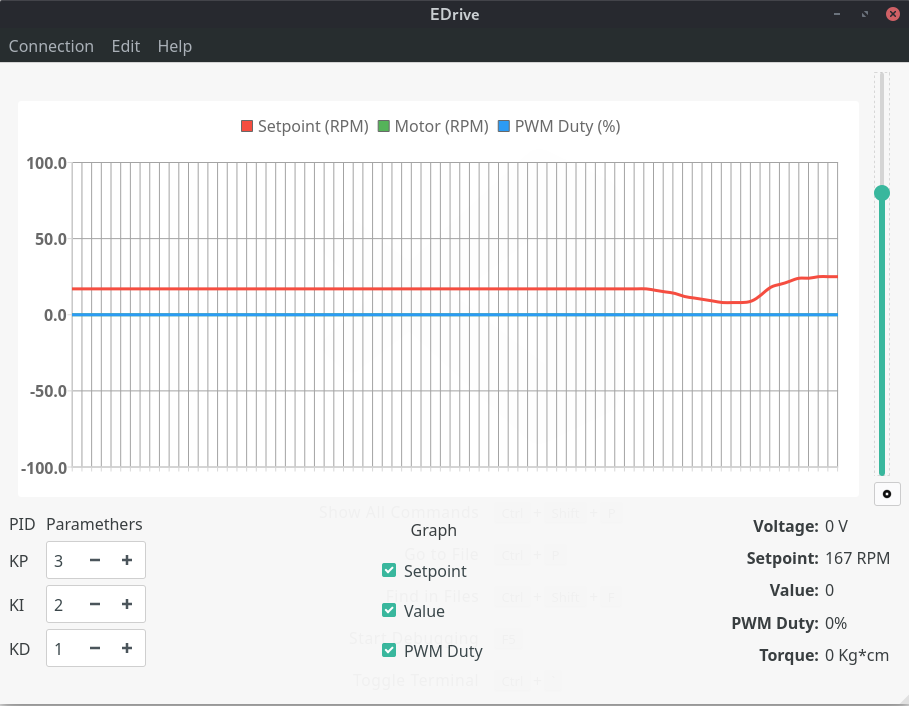
\includegraphics[width=1\textwidth]{img/app_ui.png}
        \caption{Interfejs użytkownika}
        \label{fig:app_ui}
    \end{figure}
    
    
    \subsection{Górna belka}
        W górnej części aplikacji znajduje się menu kontekstowe. Pozwala ono na wywołanie okna inicjalizującego połączenie z serwerem (patrz \ref{fig:app_connect}). Do nawiązania pomyślnego połączenia wymagane jest umieszczenie poprawnego adresu oraz portu brokera MQTT. W przypadku dezaktywowanej opcji przyjmowania anonimowych użytkowników wymagane jest także podanie ważnych danych autoryzacyjnych.
        
        \begin{figure}[ht]
            \centering
            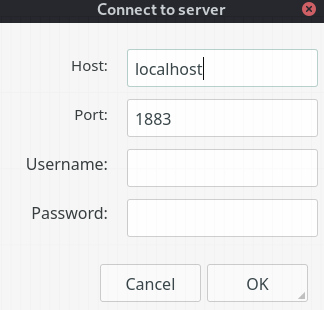
\includegraphics[width=0.5\textwidth]{img/app_connect.png}
            \caption{Okno nawiązywania połączenia}
            \label{fig:app_connect}
        \end{figure}
    
    
    \subsection{Panel parametrów}
        Dolna część okna podzielona jest na trzy części.
        
        \begin{itemize}
            \item Panel parametrów regulatora.
            \item Panel widoczności wykresów.
            \item Panel z aktualnymi danymi.
        \end{itemize}
        
        Pierwsza z nich udostępnia interfejs do dynamicznej zmiany nastaw regulatora PID. Pozwala to bardzo szybko uzyskać zadowalające nastawy, niezbędne do prawidłowego działania silnika. 
        
        Środkowy panel zawiera pola wielokrotnego wyboru służące do ukrywania niepotrzebnych danych na wykresie. Dzięki tej funkcjonalności możliwe jest uniknięcie nakładanie się na siebie wykresów, co znaczenie zwiększa komfort i czytelność prezentowanych informacji.
        
        Ostatni panel, umieszczony z prawej strony zawiera zrób danych zebranych z urządzenia wykonawczego. Można wyróżnić w śród nich:
        
        \begin{itemize}
            \item napięcie zasilanie urządzenia,
            \item ustawiony punkt pracy,
            \item aktualną prędkość obrotową silnika,
            \item wartość procentową wypełnienia PWM.
        \end{itemize}

    \subsection{Graf}
        Najatrakcyjniejszym wizualnie elementem jest wykres umieszczony w centrum okna. Wizualizuje on trzy zmienne:
        
        \begin{itemize}
            \item zadaną wartość obrotów silnika,
            \item aktualną wartość obrotów silnika,
            \item wypełnienie PWM.
        \end{itemize}
        
        Obecność wykresu umożliwia wizualną ocenę jakości sterowania.